\chapter{Miami: Access, Leverage, and the Structure of a Yes}

We are not dealing here with blackboard physics, yet the lecture does have a mathematical spine. It proceeds by contact, refusal, reset, and extraction; then, once access is secured, it turns spoken anecdotes into mechanisms. The sequence matters. We move from Miami as a field of concentrated wealth, to a food-distribution operator who turned a small acquisition into repeated nine-figure exits, to a verbal balance sheet for real-estate leverage, to John Ruiz on platform and repetition, and finally to Jordan Belfort on persuasion, qualification, and the anatomy of a real yes.

\section{Miami as a field of extraction}

The lecture opens by making Miami itself the first object of study. It is presented not as scenery but as a money hub, a place where old money, new money, millionaires, and billionaires are dense enough that one may try the same question again and again and hope eventually to penetrate the shell.

The first movement is therefore methodological. The host approaches several wealthy-looking figures and gets almost nothing: deflection, joking, gatekeeping, refusal. That is not dead material. It establishes the working rule that proximity does not itself yield knowledge. We must ask, be refused, and ask again.

The first transferable maxim of the lecture is therefore not a financial formula but a search rule: every no is a step closer to yes. In companion-note form we should keep this rule near the front, because the later business doctrine is only intelligible once we have seen the cost of access.

\section{From a \$300{,}000 purchase to repeated exits}

The first real payoff comes in the Design District with the owner of a Rolls Royce. The initial answer is compressed almost to absurdity: he got rich by selling a business. Then the lecture slows down and starts to keep a ledger.

\begin{align}
P_{\text{acq}} &= \$3 \times 10^5,\\
V_{\text{sale},1} &> \$100 \times 10^6,\\
V_{\text{sale},2} &> \$400 \times 10^6.
\end{align}

A small food-distribution business was bought for roughly \$300{,}000. It was sold once for more than \$100 million, then again, after new partners and larger management structure were brought in, for more than \$400 million. If we perform only the simplest arithmetic on the last number, we get the rough scale of the expansion:

\begin{equation}
\frac{V_{\text{sale},2}}{P_{\text{acq}}} > 1.33 \times 10^3.
\end{equation}

This is not yet a return calculation in the full financial sense; it ignores time, dilution, later investment, and financing. But it does tell us why the story arrests attention. We are meant to feel the distance between entry scale and exit scale before we are told how the distance was crossed.

\paragraph{Anecdote.}
The customers were said to be essentially all the restaurants that mattered in the market. The transcript is slightly garbled here, but the point is clear enough: the firm achieved extraordinary distribution density.

\paragraph{Mechanism.}
The lecture does not attribute this result to charisma alone. The operator names a sequence of operating necessities: the right products, the best buying team, strong procurement, a real sales force on the street, competitive pricing, and service. Service, he emphasizes, is a major factor. What we have, then, is a basic business decomposition:
\begin{itemize}
\item product quality,
\item purchasing and procurement discipline,
\item sales coverage,
\item price competitiveness,
\item service reliability.
\end{itemize}

This is the first major anti-mystical gesture in the lecture. Very large numbers are made to sit on top of ordinary commercial components.

\section{Real estate as a second engine}

The same interview then pivots from operating business to real estate. The lecturer asks where the richest people place themselves. The answer is immediate: in real estate, because if one has real estate one can never really go broke. That claim is then attached to a concrete example.

\begin{align}
P_0 &= \$5 \times 10^6, &
\alpha &\approx 0.15,\\
E_0 &\approx \alpha P_0 \approx \$7.5 \times 10^5, &
V_t &\in [\$25,\$30] \times 10^6.
\end{align}

The reported story is that a property was bought in 2013 for about \$5 million, with very little cash down, roughly fifteen percent. Today the same building is said to be worth somewhere between \$25 million and \$30 million. If we keep only the gross asset multiple, the scale is again clear:

\begin{equation}
\frac{V_t}{P_0} \in [5,6].
\end{equation}

We should state this cautiously. It is a gross appreciation ratio, not a net realized return.

\subsection{Question \& Answer}

\paragraph{Question.}
If the wealth is tied up in real estate, how do we actually use it without selling the asset?

\paragraph{Answer.}
The lecture resolves this by introducing the refinance play. Here the mathematics is elementary, but the elementary arithmetic is precisely the mechanism.

\begin{definition}
For the refinance discussion we write
\begin{equation}
E = V - D,
\end{equation}
where \(V\) is the current property value, \(D\) is the debt secured against it, and \(E\) is the equity.
\end{definition}

The spoken example is:

\begin{align}
V_0 &= \$2 \times 10^6,\\
V_t &= \$8 \times 10^6,\\
E_t &= V_t - D \approx \$8 \times 10^6 - \$2 \times 10^6 = \$6 \times 10^6.
\end{align}

The logic runs as follows.
\begin{enumerate}
\item We buy a building for \$2 million.
\item Over several years, it appreciates to \$8 million.
\item Under the simplifying assumption used in the lecture, the original \$2 million is debt.
\item The appreciated property therefore contains about \$6 million of equity.
\item Instead of selling the property, we refinance against that equity.
\item The cash thus extracted becomes deployable capital for the next purchase.
\end{enumerate}

This is what the lecturer calls the real-estate game: appreciation creates equity; equity supports borrowing; borrowing purchases more assets.

\begin{figure}
\centering
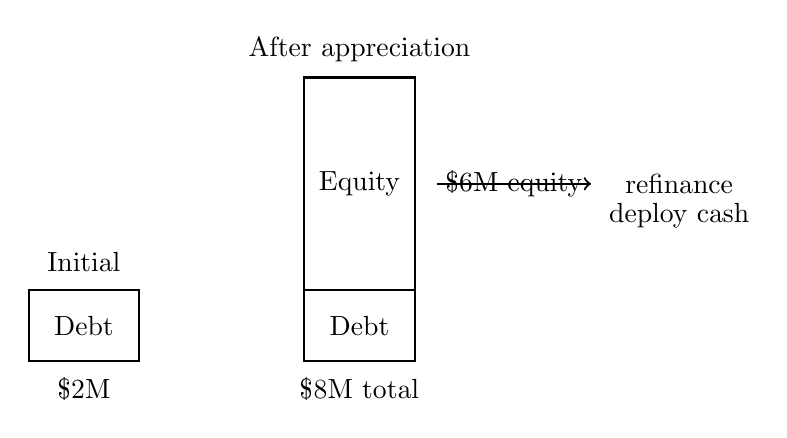
\begin{tikzpicture}[x=0.7cm,y=0.45cm]
\draw[thick] (0,0) rectangle (2,2);
\node at (1,2.8) {Initial};
\node at (1,1) {Debt};
\node at (1,-0.8) {\$2M};

\draw[thick] (5,0) rectangle (7,8);
\draw[thick] (5,2) -- (7,2);
\node at (6,8.8) {After appreciation};
\node at (6,1) {Debt};
\node at (6,5) {Equity};
\node at (6,-0.8) {\$8M total};
\node at (8.8,5) {\$6M equity};

\draw[->,thick] (7.4,5) -- (10.2,5);
\node at (11.8,5) {refinance};
\node at (11.8,4.1) {deploy cash};
\end{tikzpicture}
\end{figure}

The lecture also calls the refinance proceeds tax free. We should preserve that as a spoken claim in the notes, but not pretend that a full tax derivation has been given.

\section{Negotiation, structure, and the difference between buying and building}

Having sketched one operating machine and one leverage machine, the lecture asks for negotiation advice. The answer is simple and structural: the deal has to work for both sides. If it works only for us, it will not last; if it works only for them, we are wasting our time. The language is not mathematical, but it is bilateral. A stable deal is one in which the gain is not one-sided theater.

The same interview then moves to a different kind of structure: why people fail when selling companies, and why business formation matters from the beginning. The claim is that many sellers never built enough platform, process, or procedure to command the highest valuation. The LLC discussion, and the long promotional detour that follows, are best understood as part of the same structural argument: if we do not set the entity up correctly at the start, we handicap scale before scale begins.

\subsection{Question \& Answer}

\paragraph{Question.}
Should we buy a business or start one?

\paragraph{Answer.}
The answer given is superficially surprising. The operator says one should start, even though he himself bought a business. The resolution is that he did not buy income; he bought access.

We may write the contrast schematically as
\begin{align}
\text{purchase} &\longrightarrow \text{industry access} + \text{key employees},\\
\text{build} &\longrightarrow \text{direct use of tools, cash, and platform}.
\end{align}

This is one of the lecture's cleanest distinctions. Buying a business is not automatically the purchase of a cash stream. It may instead be the purchase of position: entry into an industry, control of relationships, and continuity of personnel. Building, by contrast, is what we do when we already possess the tools and want direct authorship of the operating machine.

\section{John Ruiz: platform, scale, and repetition}

The lecture now resets theatrically. We go to John Ruiz's compound, and the house is used as a scale marker before it becomes a subject of analysis. The point of the spectacle is not merely to impress us; it is to force the later biographical claims to move against an unmistakable measure.

The biography is sparse but strong. Ruiz says his father came from Cuba with five children and had been homeless. He was the first in the family to go to college, then to law school. He says he started with an \$800 Discover credit card and, after law school, did not have money to pay rent, so he exchanged hours of legal work for use of space. This is one of the lecture's more useful early distinctions: before one owns time, one often spends time to buy position.

\begin{align}
C_0 &= \$800,\\
V_{\text{home,now}} &\approx \$175 \times 10^6,\\
P_{\text{home}} &\approx \$46 \times 10^6.
\end{align}

The transcript then gives a garbled line about later improvements. If we normalize it conservatively as another \$20 million of capital expenditure, we obtain only a rough bookkeeping estimate:
\begin{align}
B &\approx P_{\text{home}} + I_{\text{capex}} \approx \$66 \times 10^6,\\
U &\approx V_{\text{home,now}} - B \approx \$109 \times 10^6.
\end{align}

\begin{remark}
The capex line is uncertain in the transcript, so \(B\) and \(U\) should not be treated as audited quantities. They are placeholders for scale, not a realized profit statement.
\end{remark}

The conceptual center of the Ruiz interview is not the house, however. It is the claim that the same effort is required to make \$1 as to make \$100 million, because the rules are the same and only the platform is bigger. We should not formalize that into an equality law. It is better written as a ladder of problem classes:

\begin{equation}
\$1 \longrightarrow \$10^4 \longrightarrow \$10^6 \longrightarrow \$10^9.
\end{equation}

The lecture's point is that, as we move to the right, we are not entering a new universe of laws. We are enlarging the field on which the same laws operate. At higher scale, the people on the other side move faster and understand the terrain better, but the terrain is still terrain.

Ruiz then sharpens the point further: one need not reinvent the wheel. Innovation is distinct, but most advancement at large scale is not born from perpetual originality. It comes from repeated execution on a larger platform.

He also gives a grim inventory of what that execution may cost:
\begin{align}
s &\in [3.5,4]\ \text{hours/night},\\
N_{\text{email}} &> 10^3/\text{day}.
\end{align}

These are not normative prescriptions. They are part of the lecture's effort to strip glamour from the billionaire image and replace it with availability, responsiveness, and endurance.

\section{Jordan Belfort: persuasion and the structure of a yes}

The final large case narrows the lecture from general wealth-building to persuasion. Jordan Belfort is introduced as a legend of Wall Street, but the lecture uses that legend less to retell a famous scandal than to isolate a particular skill: the ability to turn attention into commitment.

The interview opens, characteristically, with a number.

\begin{align}
Y_{\text{day,cash}} &= \$23 \times 10^6,\\
r_{\text{cash}} &\approx \frac{\$23 \times 10^6}{4\ \text{min}} \approx \$5.75 \times 10^6/\text{min}.
\end{align}

Again, we should treat the rate only as arithmetic on a spoken anecdote. The deeper point is not the per-minute number. It is that very high financial scale sits downstream from a communicative structure.

Belfort's first major doctrinal move is that every entrepreneur must be a salesperson. Not because every entrepreneur literally cold-calls prospects, but because the entrepreneur must sell a future. One sells a product, yes, but also a mission, a role, and a vision that recruits belief. His chain can be written schematically as
\begin{equation}
\text{vision} \longrightarrow \text{emotional connection} \longrightarrow \text{commitment} \longrightarrow \text{effort}.
\end{equation}

Without that chain, hiring degenerates into overpayment. The employee may take the wage but never join the mission.

\subsection{Question \& Answer}

\paragraph{Question.}
Is entrepreneurship for everyone?

\paragraph{Answer.}
At this point the lecture folds back on itself and quietly brings Ruiz and Belfort into agreement. Ruiz had already emphasized sacrifice, sleep deprivation, availability, and self-belief. Belfort now gives the other half of the answer. Entrepreneurship is not mandatory for all good lives. But for someone who wants abundance, autonomy, and the ability to choose what, when, how much, and with whom, the paycheck route is very difficult. The distinction is not between the elect and the damned. It is between different desired forms of life.

\subsection{Question \& Answer}

\paragraph{Question.}
How do we turn a no into a yes?

\paragraph{Answer.}
Belfort refuses the premise. The job of a salesperson is not to convert a genuine no into a yes. A true no means exit. The real work begins when the response is not refusal but hesitation.

We may write the decision structure as
\begin{equation}
\text{No} \longrightarrow \text{Exit},
\qquad
\text{Hesitation} \longrightarrow \text{Clarify need} \longrightarrow \text{Advance toward yes}.
\end{equation}

This is precisely why the final ``sell me this pen'' test is reversed. The bad salesperson begins with adjectives about the pen. The better salesperson begins with diagnosis. Are you even in the market for a pen? If not, the pitch is wasted motion. The lecture thus ends not with flamboyant closing technique but with qualification. Before we sell, we must know what the other side wants.

The same section also revisits money and character. Belfort says money is like alcohol: it amplifies, it does not change. Ruiz had already said that money comes and goes and that one can rebuild with drive and vision. The lecture's final moral architecture is therefore as follows: structure matters, leverage matters, persuasion matters, but beneath all of them sits a view of character under scale.

\section{Summary}

This lecture teaches by sequence rather than by theorem. We begin in a city dense with wealth, learn that access is costly, and are then shown three different mechanisms. First, a small business can become a very large exit if product, procurement, sales, and service are assembled correctly. Second, real-estate appreciation can be turned into deployable capital through equity and refinance rather than sale. Third, scale itself does not abolish ordinary commercial laws; it enlarges the platform on which they operate.

By the end, the lecture has tightened into a compact doctrine. Wealth is built through access, structure, leverage, and repetition. Persuasion is not theatrical excess but the disciplined discovery of what the other side values. And if we want the chapter's shortest mathematical slogan, it is probably this: solve larger problems on a larger platform, and the same rules begin to produce very different numbers.